\chapter{Implementacja}
\thispagestyle{chapterBeginStyle}

\section{Opis komponentów i ich połączeń}
    W programie implementującycm algorytm będący obiektem badań można wyróżnić 3 główne komponenty:
    \begin{itemize}
        \item \textbf{Algorytm} zaimplementowany w języku programowania \textbf{PROLOG}
        \item \textbf{Generator grafów} zaimplementowany w formie modułu w języku programowania \textbf{Python}
        \item \textbf{Warstwa graficzna} (GUI) zaimplementowana w języku programowania \textbf{Python} przy użyciu bibloteki \textbf{Tkinter}
    \end{itemize}
    Naistostniejszą z perspektywy użytkownika jest \textbf{Warstwa graficzna}. Jest to program, którego uruchomienie pozwala na 
    interakcję z utworzonym narzędziem w przyjazny dla użytkownika sposób. Istnieje również możliwość uruchomienia algorytmu z pominięciem 
    warstwy graficznej, o czym można dowiedzieć się więcej w sekcji \ref{CommandLine}.
    Z wyświetlonego menu użytkownik może wybrać przykładowe, wcześniej spreparowane światy, zdefiniować swój stan początkowy oraz cel (w niektórych 
    światach cel jest intuicyjny, więc jego definicja nie jest od użytkownika wymagana) i uruchomić algorytm. Wynikiem działania programu jest 
    plan, który wyświetlony jest w formie tekstowej z opisem na kroki oraz dwa grafy: graf pełen (zawierający wszystkie składowe opisane 
    w \ref{GRAPHPLANRozdzial}) oraz graf uproszczony, który zawiera jedynie niezbędne stany oraz akcje wymagane do zrozumienia wygenerowanego planu.
    Poniższy schemat klarownie przedstawia relacje między komponentami w trakcie działania programu:
    \begin{figure}[H]
        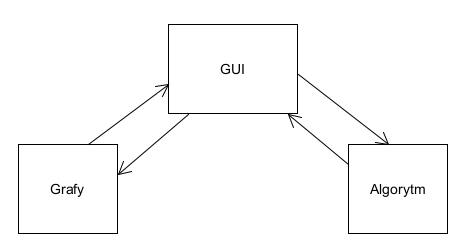
\includegraphics[scale=0.5]{zaleznosci}
        \centering
        \caption{Zależności między komponentami}
    \end{figure}
    Główna jednostką sterującą jest warstwa graficzna. W momencie naciśnięcia przez użytkownika odpowiedniego przycisku generującego rozwiązania, warstwa 
    graficzna zbiera wszystkie niezbędne informacje: w jakim świecie użytkownik pracuje, w jaki sposób zdefiniował warunki początkowe, oraz jakie cele 
    chce on uzyskać. Następnie obrobione informacje przesyłane są do algorytmu, który poza wygenerowaniem planu, do pliku tekstowego wypisuje 
    stany, akcje oraz mutexy dla każdej z warstw. Następnie algorytm przesyła swoją odpowiedź do GUI, 
    który wysyła żadanie wygenerowania grafów do odpowiednich komponentów odpowiedzialnych za ich 
    generowanie. W skład komponentu "Grafy" wchodzą dwie klasy, przy czym każda z nim generuje unikalny graf.

\section{Implementacja algorytmu}
    Algorytm \textbf{GRAPHPLAN} został zaimplementowany w języku programowania PROLOG. Poniższe diagramy przedstawiają proces  
    generowania pojedynczego planu.
    \begin{figure}[H]
        \label{PetlaGlowna}
        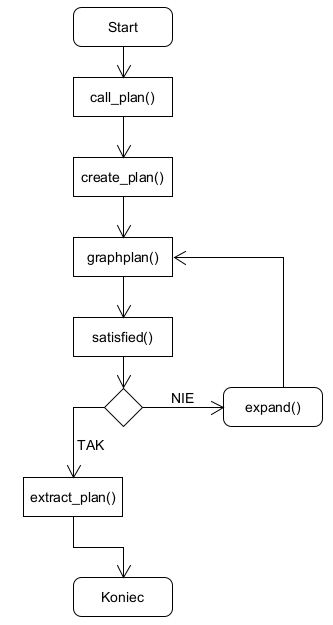
\includegraphics[scale=0.75]{GRAPHPLAN_petla_glowna}
        \centering
        \caption{Główna pętla algorytmu}
    \end{figure}

    \begin{definition}
        \label{Predykat}
        \textbf{Klauzula} -- przedstawiona informacja o świecie
    \end{definition}

    \begin{definition}
        \label{Fakt}
        \textbf{Fakt} -- informacja o świecie, która jest zawsze prawdziwa
    \end{definition}

    \begin{definition}
        \label{Regula}
        \textbf{Reguła} -- informacje, które są prawdziwe, po spełnieniu pewnych warunków
    \end{definition}

    \begin{definition}
        \label{Predykat}
        \textbf{Predykat} -- sposób wyrażania warunków w programowaniu w logice
    \end{definition}


    Przed rozpoczęciem omawiania struktury programu wprowadzono podstawowe definicje stosowane w programowaniu w logice. Przykładem klauzuli jest 
    zdanie $kobieta(anna).$ informujące program o tym, iż Anna jest kobietą. Ze względu na sposób reprezentacji danych w języku programowania PROLOG, 
    wszystkie stałe określane są małymi literami, gdyż ciągi znaków zaczynające się wielką literą zarezerwowane są dla \textit{zmiennych}. Należy 
    również zwrócić uwagę na wykorzystanie znaku przystankowego w postaci kropki (\textbf{.}), przedstawiający koniec przekazywanej informacji. 
    $kobieta(anna).$ również jest przykładem jednoargumentowego predykatu. Predykaty jednoargumentowe często określanę są mianem \textit{własności}.
    Predykaty o większej liczbie argumentów często nazywane są \textit{relacjami}. W Prologowej nomenklaturze predykaty zapisuję się zgodnie 
    z następującą strukturą: \textit{X/Y}, gdzie \textit{X} oznacza nazwę relacji (nagłówek), a \textit{Y} liczbę argumentów przyjmowaną przez 
    opisywany predykat. Zgodnie z powyższym zapis $kobieta/1$ oznacza, iż relacja kobieta przyjmuje jeden argument.
    Zdanie $kolor(brązowy).$ jest przykładem faktu, czyli zdania zawsze prawdziwego. Fakty różnią się od reguł tym, iż reguły nie muszą być zawsze prawdziwe \cite{PROLOG}.
    W sekcji \ref{DefinicjeSwiata} wprowadzono przykład reguły, wraz z opisem jej struktury.

    Założeniem działania algorytmu jest poprawne zdefiniowanie warunków początkowych oraz celów, przy użyciu wcześniej spreparowanych przez użytkownika 
    relacji. Ponadto zbiór akcji również musi zostać bezpośrednio utworzony przez użytkownika, algorytm w trakcie działania nie dokonuje żadnego 
    sprawdzenia zgodności wprowadzonych danych. Z tego powodu warstwa graficzna programu udostępnia tylko część środowisk, które zostały opisane przez 
    autora pracy zgodnie z wytycznymi języka opisu STRIPS.

    Predykat o nazwie $call\_plan/2$ odpowiada za utworzenie pliku tekstowego (nazwa pliku: \textit{output.txt}) oraz przekierowanie strumienia danych 
    do ustalonego pliku. Następnie pobiera stan świata, które zdefiniowany jest w formie faktu \textit{inital\_state/1}, który przyjmuje jeden argument
    w formie listy zawierającej wszystkie stany początkowe. Następnie dochodzi do uruchomienia predykatu $create\_plan/3$, który przyjmuje jako dane
    wejściowe początkowy stan oraz wymagany cel, a wynikiem jego działania jest utworzony plan. W tym predykacie, z pomocą predykatu $findall/3$,
    odbywa się nadanie wszystkim stanom początkowym indykatora jeden, gdyż wszystkie z tych stanów są prawdziwe w przedstawionym świecie. 
    Następnie dochodzi do wykreowania pierwszego zbioru akcji przy pomocy wbudowanego predykatu $setof/3$. Po wykreowaniu odpowiednich zbiorów 
    dochodzi do uruchomienia predykatu $graphplan/4$ - głównej pętli programu.

    \begin{listing}[H]
        \begin{minted}{prolog}
            % call_plan(+Goals,-Plan)
            call_plan(Goals,Plan) :-
                tell('outputs/output.txt'),
                inital_state(S),
                create_plan(S,Goals,Plan),
                write("Plan: "), writeln(Plan),
                told.
        \end{minted}
        \caption{Implementacja predykatu call\_plan/2}
    \end{listing}

    \begin{listing}[H]
        \begin{minted}{prolog}
            % create_plan(+StartState,+Goals,-Plan)
            create_plan(StartState, Goals, Plan) :-
                findall(State/1, member(State,StartState),StartLevel),
                setof(action(Action, Precondition, Effects), 
                (effects(Action,Effects),preconditions(Action,Precondition)),
                AllActions),
                write("StartLevel: "), write(StartLevel), nl,
                graphplan([StartLevel], Goals, Plan, AllActions).
    \end{minted}
    \caption{Implementacja predykatu create\_plan/2}
    \end{listing}

    Działanie predykatu $graphplan/4$ można podzielić na dwa etapy. W pierwszym etapie sprawdzany jest warunek konieczny utworzenia grafu- 
    obecność wszystkich stanów ze zbioru celów na aktualnym poziomie stanów. Dokonywane jest to przy pomocy predykatu $satisfied/2$, który 
    iteruje po każdym celu z listy celów i dokonuje sprawdzenia wskazanego warunku. Dodatkowo rzeczona klauzula ustala, czy indykator każdego z 
    celów jest większy od zera, czyli czy jest możliwość jego wykonania na danym poziomie stanów. Jeśli powyższe warunki są spełnione dla każdegu celu, 
    algorytm przechodzi do predykatu $extract\_plan/2$, który na podstawie aktualnego poziomu stanów 
    podejmuję próbę generowania odpowiedniego plan. 
    
    \begin{listing}[H]
        \begin{minted}{prolog}
            % graphplan(+GraphPlan,+Goals,+AllActions,-Plan)
            graphplan([StateLevel | GraphPlan], Goals, AllActions,Plan) :-
                satisfied(StateLevel, Goals),
                extract_plan([StateLevel | GraphPlan], Plan)
                ;
                expand(StateLevel, ActionLevel, NewStateLevel, AllActions),
                graphplan([NewStateLevel, ActionLevel, StateLevel | GraphPlan], 
                Goals, AllActions, Plan).
    \end{minted}
    \caption{Implementacja predykatu graphplan/4}
    \end{listing}
    
    \begin{listing}[H]
        \begin{minted}{prolog}
            % satisfied(+StateLevel, +Goals)
            satisfied(_,[]).

            satisfied(StateLevel, [G | Goals]) :-
                member(G/IG, StateLevel),
                IG #> 0,
                satisfied(StateLevel, Goals).
    \end{minted}
    \caption{Kod źródłowy implementacji predykatu satisfied/2}
    \end{listing}

    \begin{listing}[H]
        \begin{minted}{prolog}
            % extract_plan(+Graph,-Plan)
            extract_plan([_],[]).

            extract_plan([ChosenStates,ActionLevel | RestOfGraph], Plan) :-
                collect_vars(ActionLevel, AVars),
                labeling([],AVars),
                findall(A, (member(A/1,ActionLevel)),ChosenActions),
                extract_plan(RestOfGraph, RestOfPlan),
                write("ChosenActions: "), write(ChosenActions),nl,
                write("ChosenStates: "), writeln(ChosenStates),
                append(RestOfPlan, [ChosenActions], Plan).
    \end{minted}
    \caption{Implementacja predykatu extract\_plan/2}
    \end{listing}

    W przeciwnym wypadku  algorytm przechodzi do drugiej części, 
    w której dochodzi do rozszerzenia grafu planującego o kolejne warstwy przy pomocy predykatu $expand/4$. 
    Predykat $expand/4$ ma za zadanie rozszerzyć graf o kolejną warstwę. Wykonuje to korzystając z dwóch predykatów, których nazewnictwo w pełni 
    odpowiada funkcjonalności, jakie implementują. Są to- $add\_action/6$, którego zadaniem jest generowanie oraz dodawanie akcji do poziomu akcji 
    danej warstwy oraz $mutex\_state/1$ oraz $mutex\_action/2$, odpowiedzialne za tworzenie relacji wzajemnie wykluczających między stanami jak i akcjami.
    W ramach predykatu $add\_action/6$ realizowany jest również predykat $add\_effects/4$, który dla każdej akcji dodaje jej efekty do przyszłego 
    poziomu stanów.
    
    
    \begin{listing}[H]
        \begin{minted}{prolog}
        % expand(+StateLevel, -ActionLevel, -NextStateLevel, +AllActions)
            expand(StateLevel, ActionLevel, NextStateLevel, AllActions) :-
                add_actions(StateLevel, AllActions, [], NewActionLevel, [], NewNextState),
                findall(action(zostan(P),[P],[P]),member(P/_,StateLevel),PersistActs),
                add_actions(StateLevel, PersistActs, NewActionLevel, 
                ActionLevel, NewNextState, NextStateLevel),
                mutex_action(ActionLevel,NextStateLevel), 
                mutex_list(NextStateLevel),
                write("ActionLevel: "), write(ActionLevel),nl,
                write("StateLevel: "), write(NextStateLevel), nl.
    \end{minted}
    \caption{Implementacja predykatu expand/4}
    \end{listing}

    Predykat $write/1$ wykorzystywany jest wyłącznie w celu umieszczenia odpowiednich informacji o poziomie stanów oraz o poziomie akcji w pliku
    tekstowym, ktory następnie wykorzystywany jest podczas generowania odpowiednich grafów.

    \begin{listing}[H]
        \begin{minted}{prolog}
            %add_actions(+StateLevel,+Action,+PreviousActionLevel,
            -NewActionLevel,+PreviousStateLevel,-NewStateLevel)
            add_actions(_,[],ActionLevel, ActionLevel, NextStateLevel, NextStateLevel).

            add_actions(StateLevel, [action(A,Precondition,Effects) | Acts], 
            ActLev0, ActLev, NextLev0, NextLev) :-
                IA in 0..1, 
                includes(StateLevel, Precondition, IA),
                add_effects(IA, Effects, NextLev0, NextLev1), !, 
                write("A: "), write(A), nl,
                write("Precondition: "), write(Precondition), nl,
                write("Effects: "), write(Effects), nl,
                add_actions(StateLevel, Acts, [A/IA | ActLev0], ActLev, NextLev1, NextLev)
                ;
                add_actions(StateLevel, Acts, ActLev0, ActLev, NextLev0, NextLev).
    \end{minted}
    \caption{Implementacja predykatu add\_actions/6}
    \end{listing}

    Przy implementacji predykatu $add\_actions/6$ należy zwrócić uwagę na wykorzystanie programowania ograniczeń w formie zmiennej \textbf{IA}, 
    która przyjmuje wartość ze zbioru $\{0,1\}$, gdyż akcja może, ale nie musi być realizowana na danym poziomie akcji. Dodatkowo rzeczony 
    predykat korzysta z predykatu $includes/3$, który dodaje warunek na wartość przyjmowaną przez identyfikator akcji- nie może być on większy 
    niż identyfikator warunków zajścia. Należy to interpetować w następujący sposób: jeśli którykolwiek z warunków początkowych miałby w danym 
    poziomie wartość równą 0 (czyli byłby nieprawdziwy), wtedy dana akcja nie może znajdować się w planie na wskazanym poziomie, natomiast 
    prawdziwość wszystkich warunków (czyli identyfiaktora równego 1 dla każdego warunku), powoduje iż akcja znajdzie się w zbiorze potencjalnych
    akcji do wykonania na wskazanym poziomie.

    \begin{listing}[H]
        \begin{minted}{prolog}
            % includes(+StateLevel, +Preconditions, +Indykator)
            includes(_,[],_).

            includes(StateLevel, [P|Ps],IA) :-
                member(P/I, StateLevel),
                IA #=< I,
                includes(StateLevel, Ps, IA).
    \end{minted}
    \caption{Implementacja predykatu add\_actions/6}
    \end{listing}

    \begin{listing}[H]
        \begin{minted}{prolog}
            %add_effects(+Indykator,+PreviousStateLevel,-NextStateLevel)
            add_effects(_,[],StateLevel,StateLevel).

            add_effects(IA, [P | Ps], StateLev0, ExpandedState) :-
                (remove(P/IP,StateLev0,StateLev1),!,
                NewIP #= IP+IA,
                StateLevel = [P/NewIP | StateLev1]
                ;
                StateLevel = [P/IA | StateLev0], !
                ),
                add_effects(IA, Ps, StateLevel, ExpandedState).
    \end{minted}
    \caption{Implementacja predykatu add\_effects/4}
    \end{listing}
    
    
    Następnie, w celu zachowania spójności, dla utworzonych zbiorów 
    generowane są relacje wzajemnego wykluczania określone mianem \textit{mutex'ów}. Mechanizm mutex'ów implementowany jest przy pomocy dwóch predykatów:
    \begin{itemize}
        \item \textbf{mutex\_state/1} - predykat odpowiedzialny za ustalenie, które stany znajdują się w relacji wykluczającej na wskazanym 
        poziomie generowania planu
        \item \textbf{mutex\_action/2} - predykat odpowiedzialny za ustalenie, które akcje znajdują się w relacji wykluczającej na wskazanym
        poziomie generowania planu. Dodatkową funkcjonalnością rzeczone predykatu jest ustalenie mutex'ów między efektami akcji, które 
        nie zawsze muszą być objęte definicjami wprowadzonymi w ramach \textbf{mutex\_state/1}.
    \end{itemize}

    Działanie predykatów jest bardzo zbliżone z tą różnicą, iż operują na innych obiektach. Schemat działania prezentuje się w sposób następujący:
    \begin{enumerate}
        \item Ustal element ze zbioru stanów
        \item Następnie dobierz do pary każdy z pozostałych elementów poziomu stanów i sprawdź, czy ów stany wykluczają się wzajemnie
        \item Wróć do pierwszego kroku, jako element ustalając następny obiekt wchodzący w skład listy stanów
    \end{enumerate}

    Powyższy opis został zaprezentowant z perspektywy predykatu \textbf{mutex\_state/1}. Dla predykatu \textbf{mutex\_action/2} jedyną różnicą jest 
    dodatnie ostatniego kroku, w którym wszystkie efekty wskazanych akcji zostają ze sobą połączone relacją wzajemnie wykluczającą. Determinowane 
    jest to uniknięciem sytuacji określanej w sekcji \ref{WzajemneWykluczanieRozdzial} jako \textbf{niespójny efekt}.

    \begin{listing}[H]
        \begin{minted}{prolog}
            %mutex_state(StateLevel)
            mutex_state([]).

            mutex_state([P | Ps]) :-
            mutex_single(P,Ps),
            mutex_state(Ps).
    \end{minted}
    \caption{Implementacja predykatu mutex\_state/1}
    \end{listing}

    \begin{listing}[H]
        \begin{minted}{prolog}
            %mutex_single(+State,+StateLevel)
            mutex_single(_,[]).

            mutex_single(P/I, [P1/I1 | Rest]) :-
                ( mutex(P,P1), !, I*I1 #= 0
                ;
                true
                ),
                mutex_single(P/I,Rest).
    \end{minted}
    \caption{Implementacja predykatu mutex\_single/2}
    \end{listing}

    Przy implementacji predykatu \textbf{mutex\_single/2} należy zwrócić uwagę na moment, w którym dwa stany zostały uznane przez algorytm jako
    wykluczające. Wtedy dochodzi do ustalenia ograniczenia na indykatory tych zmiennych w postaci $I*I1 \#= 0$, co znaczy, iż wspomniane dwa 
    stany nie mogą jednocześnei występować w danej iteracji świata (jeśli istniałyby, to każdy z tych stanów miałby indykator równy 1, a $1*1=1$, 
    co jest sprzeczne z ustalonym ograniczeniem)

    \begin{listing}[H]
        \begin{minted}{prolog}
            %mutex(+State1,+State2)
            mutex(P,~P) :-
            write("Mutex: ["), write(P), write(","),write(~P), writeln("]"),!.
        
        mutex(~P,P) :-
            write("Mutex: ["), write(~P), write(","),write(P), writeln("]"),!.  
        
        mutex(A,B) :-              
            inconsistent(A,B),
            write("Mutex: ["), write(A), write(","),write(B), writeln("]"), 
            !.
    \end{minted}
    \caption{Implementacja predykatu mutex/2}
    \end{listing}

    Warunki wykluczania stanów wynikają wprost z informacji zawartych w sekcji \ref{WzajemneWykluczanieRozdzial}. Predykat $incosistent/2$ jest bezpośrednio definiowany przez 
    użytkownika w ramach ustalania warunków zachodzących w rozpatrywanym świecie.

    W przypadku generowania wykluczeń dla akcji należy jedynie wspomnieć o predykatach: $mutex\_for\_action/3$, $mutex\_all\_states/3$ oraz $apply\_mutex/4$.
    Pozostałe predykaty, mimo posiadania innych nazw, działają identycznie względem predykatów utworzonych na rzecz ustalania relacji wykluczającej dla 
    pary stanów.

    \begin{listing}[H]
        \begin{minted}{prolog}
            %mutex_for_action(+Action1,+Action2,+StateLevel)
            mutex_for_action(A1,A2,StateLevel) :-
            (preconditions(A1,Precondition),effects(A2,Effects)
            ;
            preconditions(A2,Precondition),effects(A1,Effects)
            ),
            member(P1,Precondition),
            member(P2,Effects),
            mutex(P1,P2),
            write("Mutex: ["), write(A1), write(","),write(A2), writeln("]"),
            mutex_all_states(A1,A2,StateLevel),
            !.
    \end{minted}
    \caption{Implementacja predykatu mutex\_for\_action/3}
    \end{listing}

    Predykat \textbf{mutex\_for\_action/3} sprawdza, czy dwie akcje sobie nie przeszkadzają (przeszkadzanie jest jednym z przypadków, który determinuje 
    wykluczenie dwóch akcji. Więcej w sekcji \ref{WzajemneWykluczanieRozdzial}) przez sprawdzenie, czy warunki zajścia jednej z akcji nie kolidują 
    z efektami drugiej.
    \begin{listing}[H]
        \begin{minted}{prolog}
            %mutex_all_state(+Action1,+Action2,+StateLevel)
            mutex_all_states(A1,A2,StateLevel) :-
            effects(A1,E1),
            effects(A2,E2),
            findall([X,Y],(member(X,E1),member(Y,E2)),C),
            apply_mutex(C,A1,A2,StateLevel).
    \end{minted}
    \caption{Implementacja predykatu mutex\_all\_states/3}

    Jeśli dwie akcje są ze sobą w relacji wykluczającej to ich efekty także muszą się w niej znaleźć. Wykonywane jest to przy pomocy powyższego 
    predykatu \textbf{mutex\_all\_states/3}, który zbiera efekty dwóch akcji, tworzy z nich iloczyn kartezjański przy pomocy predykatów 
    $findall/3$ oraz $member/2$. Wygenerowany iloczyn przekazuje do predykatu \textbf{apply\_mutex/4}, którego zadaniem jest wygenerowanie 
    odpowiednich ograniczeń względem wskazanego zbioru efektów.
    \end{listing}

    \begin{listing}[H]
        \begin{minted}{prolog}
            %apply_mutex(+EffectsSet, +A1,+A2,+StateLevel)
            apply_mutex([],_,_,_).

            apply_mutex([H | T], A1/I1,A2/I2,StateLevel) :-
                [First,Second] = H, 
                member(First/F,StateLevel),
                member(Second/S,StateLevel),
                F*S #=< I1*I2,
                write("Mutex: ["), write(First), write(","),write(Second), writeln("]"),
                apply_mutex(T,StateLevel).
            !.
    \end{minted}
    \caption{Implementacja predykatu apply\_mutex/4}
    \end{listing}
    Należy zauważyć, iż indykatory efektów są ściśle uzależnione od wskaźników akcji, z których podchodzą ($F*S \#=< I1*I2$).

    Zakończenie generowania mutex'ów dla wszystkich stanów oraz akcji oznacza ukończenie generowania kolejnej warstwy grafu przez algorytm. 
    Następnie dochodzi do rekurencyjnego wywołania predykatu $graphplan/4$ w celu rozszerzenia grafu o kolejną warstwę. Procedura ta 
    jest powtarzana aż do momentu wygenerowania przez predykat $extract\_plan/2$ odpowiedniego planu.


\section{Generowanie grafów}
    Moduł generowania grafów utworzony w języku programowania \textbf{python} przy użyciu biblioteki \textbf{graphviz}, zgodnie ze swoją nazwą,
    przeznaczony jest do generowania grafów na podstawie otrzymanych informacji od algorytmu.
    \subsection{Struktura pliku tekstowego}

    \begin{lstlisting}
        Struktura pliku tekstowego
    \end{lstlisting}

    \subsection{Graf prosty}

    \begin{figure}[H]
        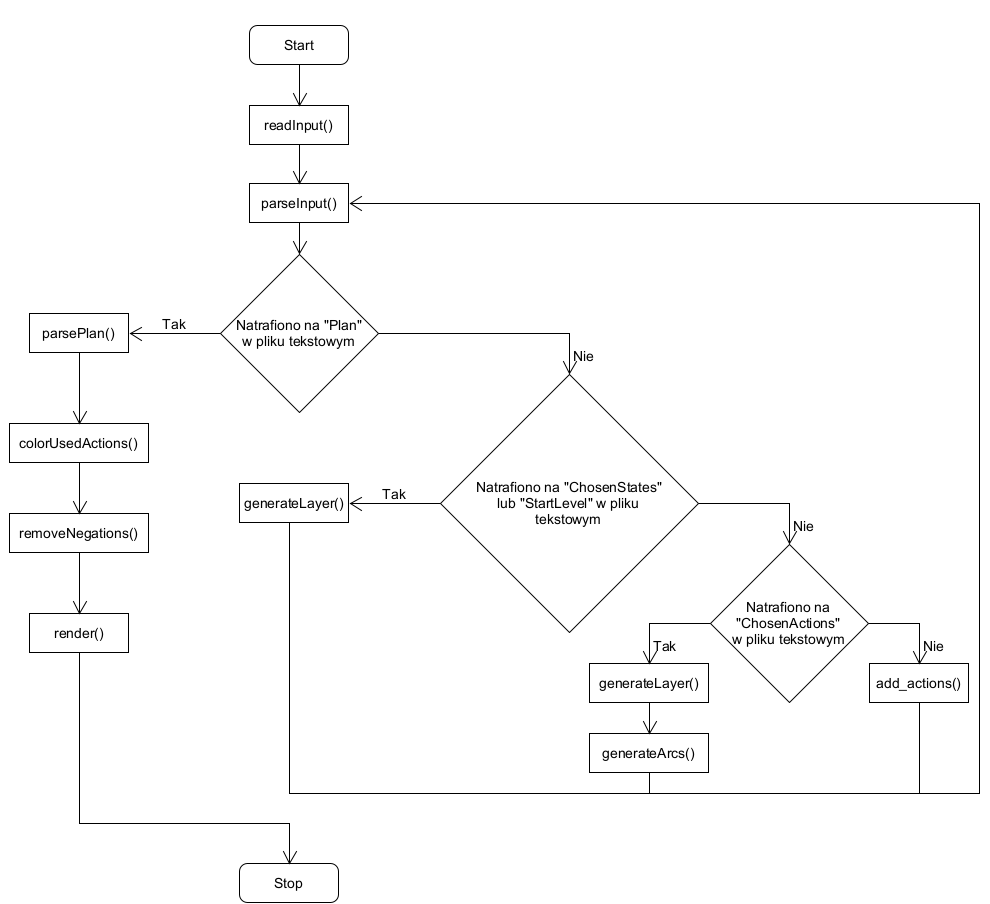
\includegraphics[scale=0.5]{UML_simplified}
        \centering
        \caption{Diagram przepływu dla generowania pojedynczego grafu prostego}
    \end{figure}

    \subsection{Graf pełny}



\section{Interfejs użytkownika}
    Interfejs użytkownika wykonany w języku \textbf{python} stanowi spoiwo, łącząc w sobie wygenerowany plan przez algorytm oraz wygenerowane grafy przez 
    odpowiedni moduł. Poniższa rycina przedstawia w sposób ogólny diagram przepływu w trakcie obsługi programu przez użytkownika:

    //Tutaj rysunek + opis ważniejszych funkcji


\section{Uruchomienie algorytmu z linii komend}
    \label{CommandLine}
    Zalecanym sposobem uruchomienia algorytmu jest wykorzystanie specjalnie przygotowanego programu graficznego, jednakże implementacja zezwala na 
    wykonywanie planów z linii komend. Ów funkcjonalność została wykorzystana między innymi w testach, których opis można znaleźć w ostatnim rozdziale pracy.
    //Jak odpalić z terminala + co należy dodać
